%-----------------------------------LICENSE------------------------------------%
%   This file is part of Mathematics-and-Physics.                              %
%                                                                              %
%   Mathematics-and-Physics is free software: you can redistribute it and/or   %
%   modify it under the terms of the GNU General Public License as             %
%   published by the Free Software Foundation, either version 3 of the         %
%   License, or (at your option) any later version.                            %
%                                                                              %
%   Mathematics-and-Physics is distributed in the hope that it will be useful, %
%   but WITHOUT ANY WARRANTY; without even the implied warranty of             %
%   MERCHANTABILITY or FITNESS FOR A PARTICULAR PURPOSE.  See the              %
%   GNU General Public License for more details.                               %
%                                                                              %
%   You should have received a copy of the GNU General Public License along    %
%   with Mathematics-and-Physics.  If not, see <https://www.gnu.org/licenses/>.%
%------------------------------------------------------------------------------%
%   Author:     Ryan Maguire                                                   %
%   Date:       September 29, 2023                                             %
%------------------------------------------------------------------------------%
\documentclass{beamer}
\usepackage{graphicx}
\usepackage{amsmath}
\graphicspath{{../images/}}
\title{Legendre Polynomials and Saturn}
\author{Ryan Maguire}
\date{September 29, 2023}
\usenavigationsymbolstemplate{}
\setbeamertemplate{footline}[frame number]
\begin{document}
    \maketitle
    \begin{frame}{Outline}
        \begin{itemize}
            \item The Cassini Mission
            \item Fourier Optics and the Fresnel Transform
            \item The Fresnel Approximation
            \item Legendre Polynomials
        \end{itemize}
    \end{frame}
    \begin{frame}{The Cassini Mission}
        \begin{figure}
            \resizebox{\textwidth}{!}{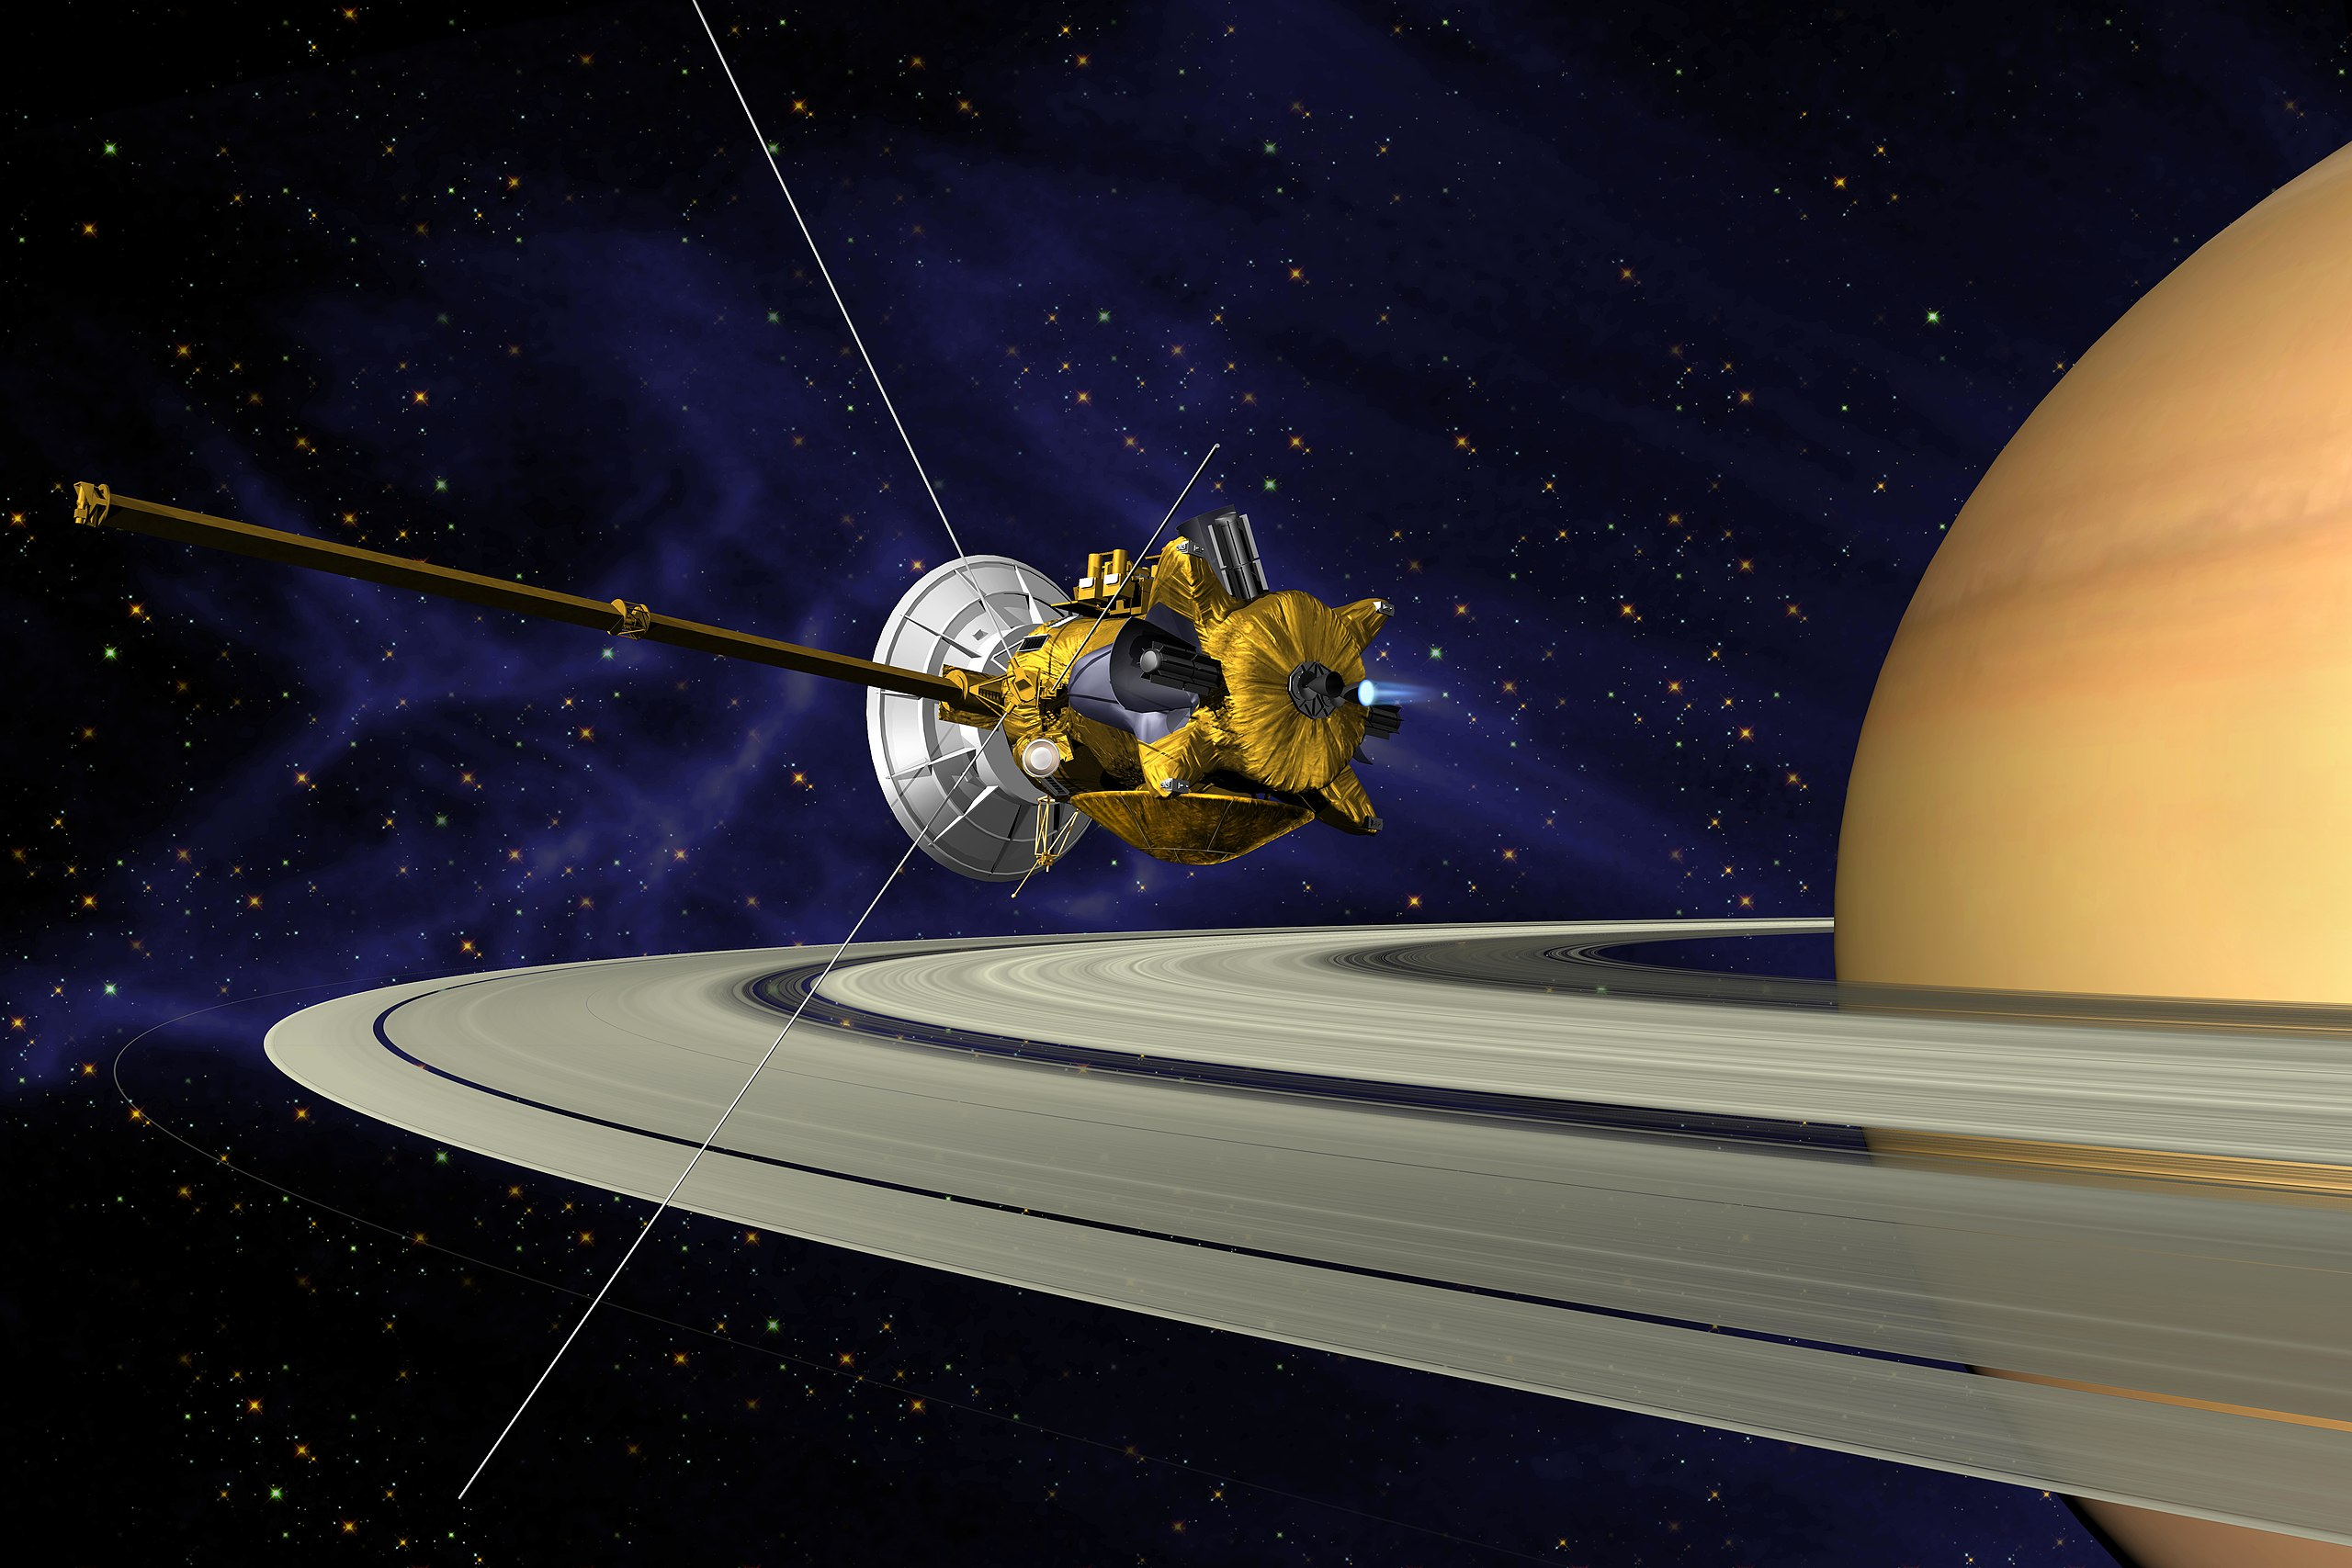
\includegraphics{cassiniorbiter.jpg}}
        \end{figure}
    \end{frame}
    \begin{frame}{The Cassini Mission}
        The Cassini orbiter was a space probe sent to Saturn back in the 90s.
        Launched in 1997, it took about 7 years to get there, arriving in 2004
        (the distance to Saturn is about 1 billion miles).
        \par\hfill\par
        Before burning up in the atmosphere of Saturn, Cassini spent 13 years
        orbiting the planet collecting data on the rings, poles, and more.
        In this talk we'll discuss some of the details of the radio science
        mission.
    \end{frame}
    \begin{frame}{The Cassini Mission}
        As Cassini orbited Saturn, occasionally its rings got between the
        the probe and Earth. This phenomenon is called an \textit{occultation}.
        Radio waves sent to Earth are then diffracted by the rings, and one
        observes a diffraction pattern on Earth. The goal is to reconstruct
        the ring profile from this diffracted pattern using Fourier optics.
    \end{frame}
    \begin{frame}{Fourier Optics and the Fresnel Transform}
        The rings of Saturn are very circular, so the
        \textit{optical transmittance} can be approximated by
        $T(\rho,\,\phi)=T(\rho)$, where $\phi$ is the azimuth angle in the
        ring plane, and $\rho$ is the radial distance from a point in the
        plane to the core of Saturn. Fourier optics tells us that the
        diffracted profile can be computed via:
        \begin{equation}
            \hat{T}(\rho_{0})=
                \int_{0}^{\infty}\int_{0}^{2\pi}
                    \rho{T}(\rho)
                    \frac{e^{i\psi(\rho,\,\rho_{0},\,\phi,\,\phi_{0})}}{D}
                    \textrm{d}\rho\,\textrm{d}\phi
        \end{equation}
        where $D$ is the distance from the point $(\rho,\,\phi)$ to the
        observer (the Cassini probe), and $\psi$ is the
        \textit{Fresnel kernel}.
    \end{frame}
    \begin{frame}{Fourier Optics and the Fresnel Transform}
        This double integral is quite hard to work with, but can be approximated
        by a single integral using the \textit{stationary phase approximation}.
        We observe for an integral of the form:
        \begin{equation}
            I=\int_{a}^{b}e^{i\phi(t)}\textrm{d}t
        \end{equation}
        where $\phi$ grows faster-than-linear, most of the contribution comes
        from where $\phi$ is roughly stationary. That is, as $\phi$ grows
        faster and faster, $e^{i\phi(t)}$ starts to oscillate rapidy, meaning
        the regions under the curve start to cancel each other out and
        contribute little to the integral.
    \end{frame}
    \begin{frame}{Fourier Optics and the Fresnel Transform}
        By applying this to the Fresnel transform, we get:
        \begin{equation}
            \hat{T}(\rho_{0})=K\int_{0}^{\infty}
                T(\rho)e^{i\psi(\rho,\phi_{s},\rho_{0},\phi_{0})}\textrm{d}\rho
        \end{equation}
        where $\phi_{s}$ is the \textit{stationary value} of $\psi$, where
        $\partial\psi/\partial\phi$ is zero, and $K$ is (roughly) some constant.
        $\hat{T}$ is the measured quantity, and $T$ is the transmittance of the
        rings, the value we wish to solve for. These \textit{integral equations}
        generally yield very hard inverse problems. We try some approximations.
    \end{frame}
    \begin{frame}{Fourier Optics and the Fresnel Transform}
        The Fresnel kernel has the form:
        \begin{equation}
            \psi=kD\Big(\sqrt{1-2\xi+\eta}+\xi-1\Big)
        \end{equation}
        where:
        \begin{align}
            \xi&=
            \frac{\cos(B)}{D}\big(\rho\cos(\phi)-\rho_{0}\cos(\phi_{0})\big)\\
            \eta&=
            \frac{\rho^{2}+\rho_{0}^{2}-2\rho\rho_{0}\cos(\phi-\phi_{0})}{D^2}
        \end{align}
        Where $B$ is the angle made with the ring plane and the line from
        the observer (Cassini) to the detector (Earth).
    \end{frame}
    \begin{frame}{The Fresnel Approximation}
        A decent approximation to the stationary value $\phi_{s}$ is
        $\phi_{s}=\phi_{0}$. We can improve this by applying one iteration of
        Newton's method to the Fresnel kernel $\psi$. This yields the
        \textit{Fresnel approximation}. The constant and linear term for
        $\psi$ ends up being zero, and by truncating the power series for
        $\psi$ to the quadratic we get:
        \begin{equation}
            \hat{T}(\rho_{0})=K\int_{0}^{\infty}
                T(\rho)e^{i\frac{\pi}{2}\big(\frac{\rho-\rho_{0}}{F}\big)^{2}}\textrm{d}\rho
        \end{equation}
        where $F$ is the so-called \textit{Fresnel scale}. The constant $K$ can
        be expressed in terms of the Fresnel scale as well, yielding:
        \begin{equation}
            \hat{T}(\rho_{0})=\frac{1-i}{F}\int_{0}^{\infty}
                T(\rho)e^{i\frac{\pi}{2}\big(\frac{\rho-\rho_{0}}{F}\big)^{2}}\textrm{d}\rho
        \end{equation}
    \end{frame}
    \begin{frame}{The Fresnel Approximation}
        As long as $F$ can be treated as constant (a usually safe assumption),
        this final equation is a \textit{convolution} of $T$ with the
        simplified Fresnel kernel. The convolution theorem, which states that
        the Fourier transform of a convolution is the product of the
        individual Fourier transforms, then tells us how to invert this
        equation for $T$. We get:
        \begin{equation}
            T(\rho)=\frac{1+i}{F}\int_{0}^{\infty}
                \hat{T}(\rho_{0})e^{-i\frac{\pi}{2}\big(\frac{\rho-\rho_{0}}{F}\big)^{2}}\textrm{d}\rho_{0}
        \end{equation}
        Note the similarity of this inversion with the Fourier transform.
        The Fresnel transform and the Fourier transform are very closely
        related.
    \end{frame}
    \begin{frame}{The Fresnel Approximation}
        For certain geometrical scenarios the approximation does not hold and
        one has to perform something like Newton's method or Halley's method
        to get an accurate value for the stationary phase approximation.
        \par\hfill\par
        This is slow. We use Legendre polynomials to speed up this calculation.
    \end{frame}
    \begin{frame}{Legendre Polynomials}
        Legendre polynomials are defined as an \textit{orthogonal} system of
        polynomials on the interval $[-1,\,1]$. That is, $P_{n}(x)$ is a
        sequence of polynomials satisfying:
        \begin{equation}
            \int_{-1}^{1}P_{n}(x)P_{m}(x)=0
        \end{equation}
        whenever $n\ne{m}$. The Sturm-Liouville equation that defines them is:
        \begin{equation}
            (1-x^{2})P_{n}''(x)-2xP_{n}'(x)+n(n+1)P_{n}(x)=0
        \end{equation}
    \end{frame}
    \begin{frame}{Legendre Polynomials}
        The generating function of the Legendre polynomials is:
        \begin{equation}
            \sum_{n=0}^{\infty}P_{n}(x)t^{n}
                =\frac{1}{\sqrt{1-2xt+t^{2}}}
        \end{equation}
        We're seen something like this already. Recall the formula for the
        Fresnel kernel:
        \begin{equation}
            \psi=kD\Big(\sqrt{1-2\xi+\eta}+\xi-1\Big)
        \end{equation}
        The partial derivative of $\psi$ with respect to $\phi$, evaluated at
        $\phi=\phi_{0}$, can then be represented via the derivative of the
        generating function. In particular, the stationary value can be
        efficiently approximated by Legendre polynomials.
    \end{frame}
    \begin{frame}{Legendre Polynomials}
        By using quartic or octic expansions, we can roughly the same speed as
        the quadratic Fresnel approximation, but still be able to apply the
        approximation in more extreme geometries (such as low $B$ values).
        The speed improvements over the full Newton-method computation is about
        100x or more, depending on the data set.
    \end{frame}
\end{document}
